\section{Méthode de fabrication du capteur}
\label{chap:capteur}
Les capteurs, constitués de la membrane nanoporeuse, des électrodépositions ainsi que des dépôts physiques en phase vapeur d'or (\gls{pvd}) sont 
fabriquées avec plusieurs membranes différentes et selon 2 méthodes :

\subsection{Membranes à disposition}
\begin{table}[H]
    \centering
    \begin{tabular}{|c|p{3cm}|c|p{3cm}|p{2cm}|p{2cm}|}
        \hline
        Membrane & Épaisseur de la membrane [$\upmu$m] & Matériau      & Densité des pores [cm$^2$] & Diamètre des pores [nm] & Porosité de surface \\
        \hline
        GTTP     & 25                                  & Polycarbonate & $1.8 \cdot 10^8$           & 220                     & 13.7 \%             \\
        \hline
        VCTP     & 25                                  & Polycarbonate & $2.7 \cdot 10^8$           & 100                     & 4.2 \%              \\
        \hline
        PI25005  & 25                                  & Polyimide     & $1 \cdot 10^8$             & 50                      & 0.4 \%              \\
        \hline
    \end{tabular}
    \caption{Matériau des membranes disponibles}
    \label{tab:membranes}
\end{table}

Le tableau \ref{tab:membranes}, montre les paramètres des membranes commerciales (sociétés Millipore et IT4IP) utilisées dans ce projet.\\
Ces membranes sont traversées de nanopores parallèles dans le sens de l'épaisseur. Les densités et diamètres des pores sont rappelés dans le 
tableau. 

\subsection{Électrodéposition de nanofils}
Ces membranes vont être dotées de vias de nanofils thermoélectriques en suivant les étapes ci-dessous. \\

Un côté de la membrane va être recouvert d'une fine couche d'or (environ 100 nm) par technique de dépôt physique en phase vapeur (\gls{pvd}). 
Le couche d'or sert d'électrode de travail pour une déposition électrochimique de Tellure de Bismuth à l'intérieur des pores comme illustré sur 
la figure \ref{fig:electrodeposition}. La technique d'électrodéposition (\gls{ed}) est détaillée dans la référence \cite{gravier_low-cost_2021}. 
L'électrolyte utilisé ici est une solution aqueuse de 200 mL contenant 0.04 mol/L de tellure [Te$^0$] et de 0.02 mol/L de 
Bi(HNO$_3$)$_3\,\cdot$ 5H$_2$O dilué dans 2 mol/L de HNO$_3$ à 65\%. \\
L'\gls{ed} s'effectue sous un potentiel de réduction cathodique de 70 mV par rapport à une électrode de référence Ag/AgCl. 

\begin{figure}[H]
    \centering
    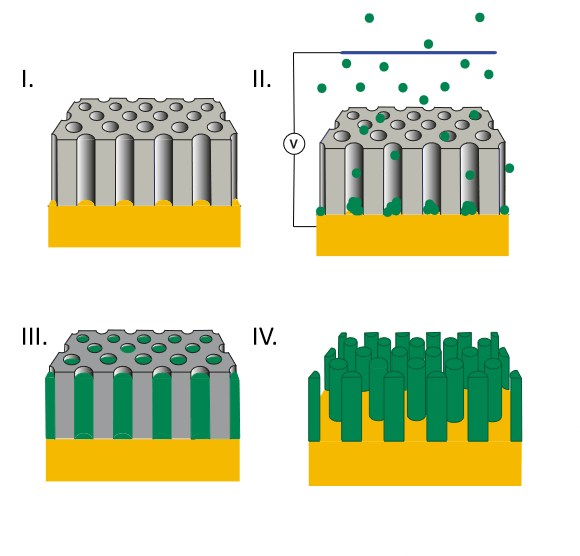
\includegraphics[scale = 0.4]{images/Electrodeposition.png}
    \caption{Électrodéposition}
    \label{fig:electrodeposition}
\end{figure}

Chaque pore rempli forme une aiguille appelée nanofil. Pour la présente application, les nanofils sont regroupés en vias de 1 mm de 
diamètre. Le coefficient Seebeck des vias a été mesuré autour de -65 $\upmu$V/K. \\
Le temps d'\gls{ed}, décide de l'importance de la croissance à la surface de la membrane, nommée par la suite, surcroissance. 

Le fonctionnement du débitmètre pédiatrique combine la nanotechnologie et l'effet de Seebeck. \\
En effet, un corps de chauffe est placé entre deux couches d'or en forme de L (cf. figure \ref{fig:schema_global}). Chaque extrémité du "L" est 
dotée d'un via de nanofils de tellure de bismuth, les vias étant court-circuités entre eux par un dépôt d'or au dos de la membrane (cf. figure 
\ref{fig:schema_coupe}). L'ensemble forme un dispositif de thermocouples mesurant la différence de température entre les surcroissances de chaque "L".\\
Lorsqu'un courant viendra 
alimenter la piste d'or du milieu, celle-ci va s'échauffer. Une différence de température va se créer entre les deux pistes d'or en "L" lorsque 
le patient viendra expirer ou inspirer de l'air sur le corps de chauffe (figures \ref{fig:schema_coupe} et \ref{fig:sensirion}). 
\begin{figure}[H]
    \centering
    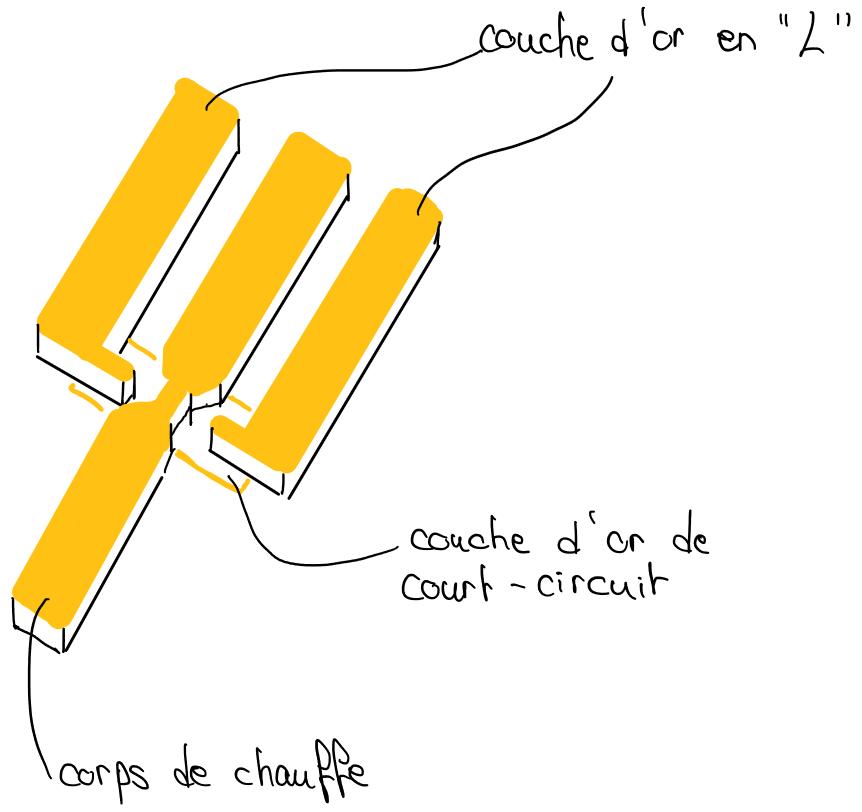
\includegraphics[scale = 0.4]{assets/figures/schema_capteur_vue_generale.png}
    \caption{Schéma du capteur - Vue globale}
    \label{fig:schema_global}
\end{figure}
\begin{figure}[H]
    \hspace{-0.7cm}
    \begin{subfigure}{0.4\textwidth}
        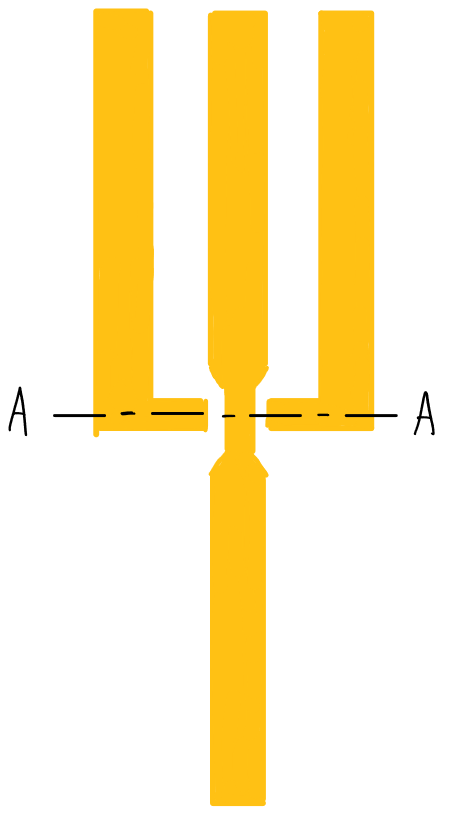
\includegraphics[scale = 0.3]{assets/figures/schema_capteur_vue_dessus.png}
        \caption{Schéma du capteur - Vue de dessus}
        \label{fig:schema_dessus}
    \end{subfigure}
    \begin{subfigure}{0.4\textwidth}
        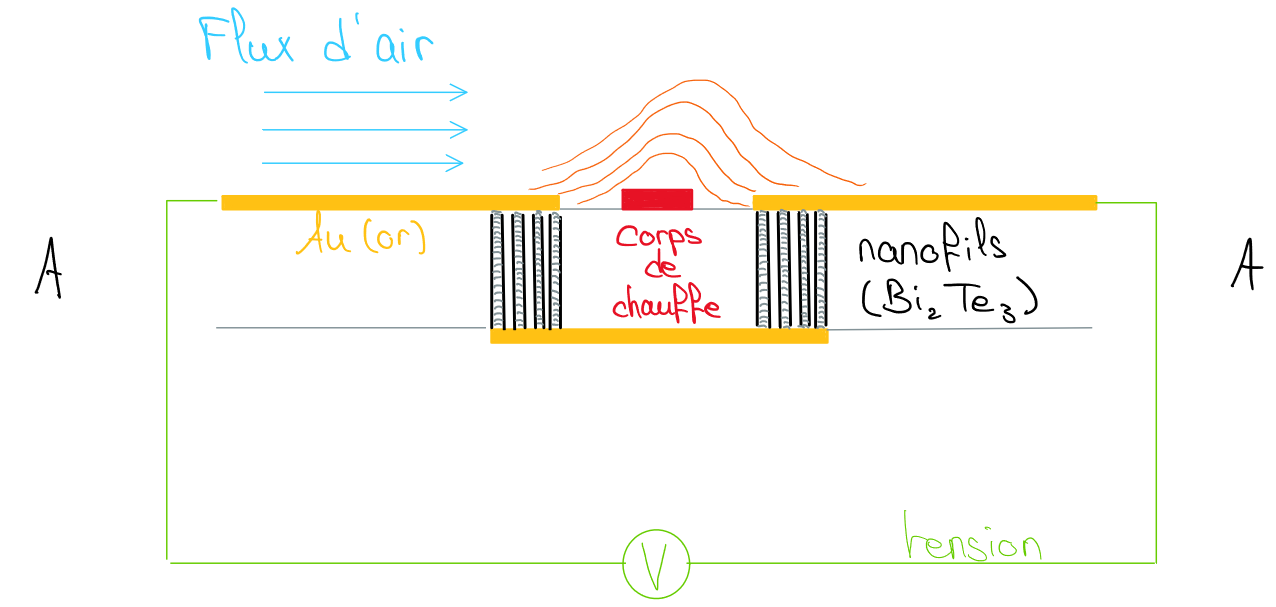
\includegraphics[scale = 0.4]{images/CapteurFUN.png}
        \caption{Schéma de principe du débitmètre nanostructuré}
        \label{fig:schema_coupe}
    \end{subfigure}
    \caption{Schéma du capteur - Vue de dessus et en coupe}
\end{figure}
Nous pouvons observer sur la figure \ref{fig:schema_coupe} que plusieurs électrodépositions (\gls{ed}) sont faites (à l'endroit des nanofils). Une première 
se situe à gauche du corps de chauffe et la deuxième, à sa droite. \\
Avec une différence de température de part et d'autre du corps de chauffe, un courant va circuler entre la couche d'or en "L" de gauche, à 
travers les nanofils gauches, au sein de la couche d'or du bas (couche d'or de court-circuit) puis dans les nanofils de droite (circuit du thermoélectrique). 
Une tension va apparaître et il sera alors possible de lier cette tension au débit inspiré et expiré du nouveau-né.\\
Cette membrane nanoporeuse associée des différentes électrodépositions et couches d'or sera appelée capteur \gls{capteur}. 

Étant donné que les nanopores sont extrêmement fins et courts, il est attendu d'obtenir un temps de réponse très intéressant (temps 
de réponse faible). 

\newpage
\subsection{Méthode A et B}
Les capteurs ont été conçus soit par la méthode A, soit par la méthode B. Ces méthodes sont expliquées dans les paragraphes qui suivent :
\begin{itemize}
    \item \textbf{Méthode A}
          \begin{figure}[H]
              \centering
              \begin{subfigure}{0.45\textwidth}
                  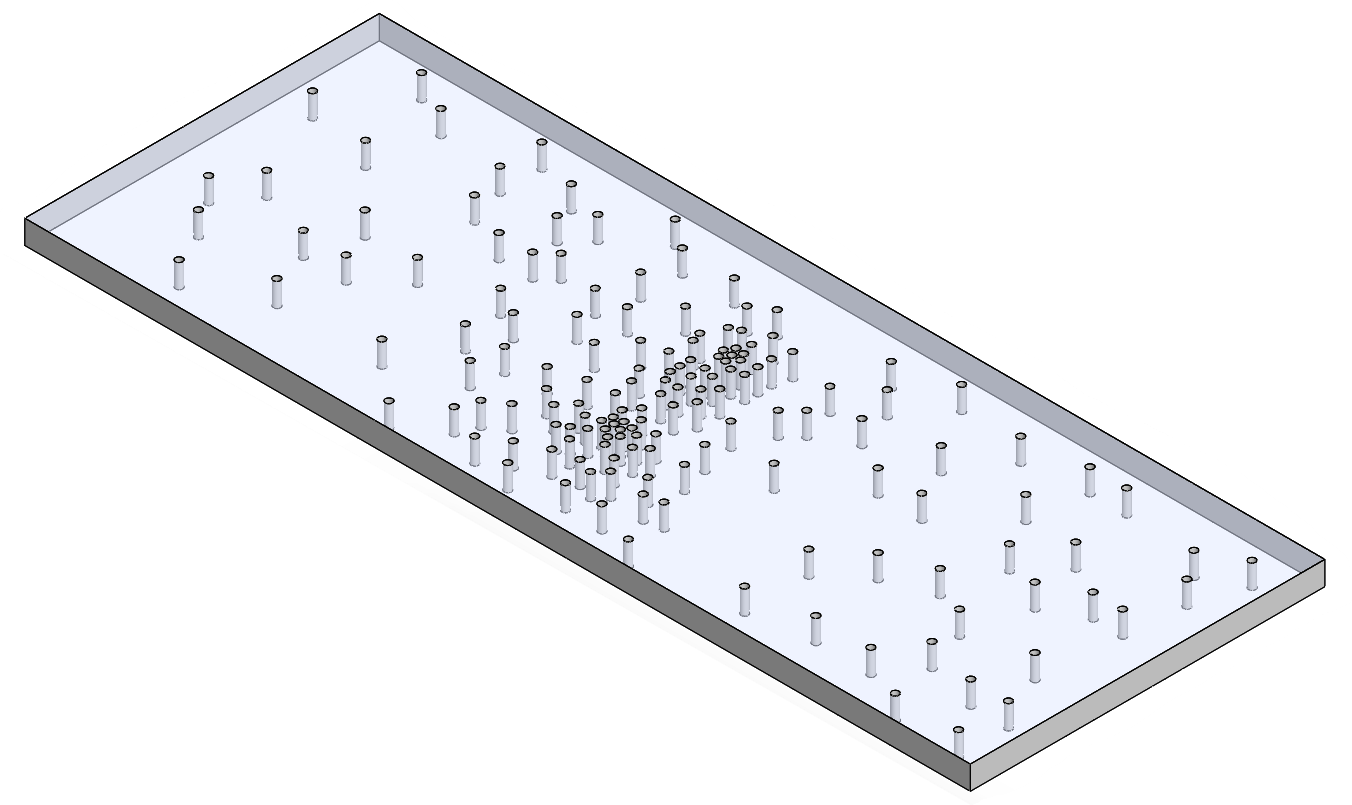
\includegraphics[scale = 0.22]{assets/figures/Membrane_nue.png}
                  \caption{Membrane nanoporeuse}
              \end{subfigure}
              \begin{subfigure}{0.45\textwidth}
                  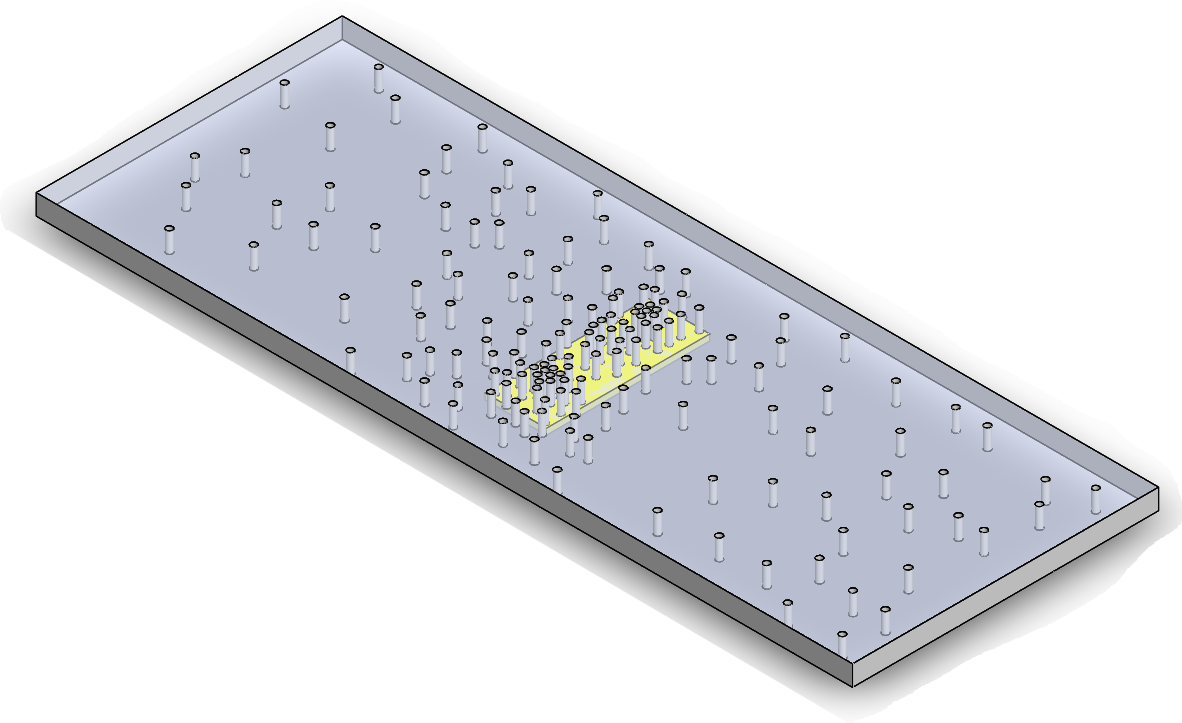
\includegraphics[scale = 0.27]{assets/figures/Court_circuit.png}
                  \caption{Dépôt physique en phase vapeur (PVD) d'or du court-circuit}
              \end{subfigure}
              \newline
              \begin{subfigure}{0.45\textwidth}
                  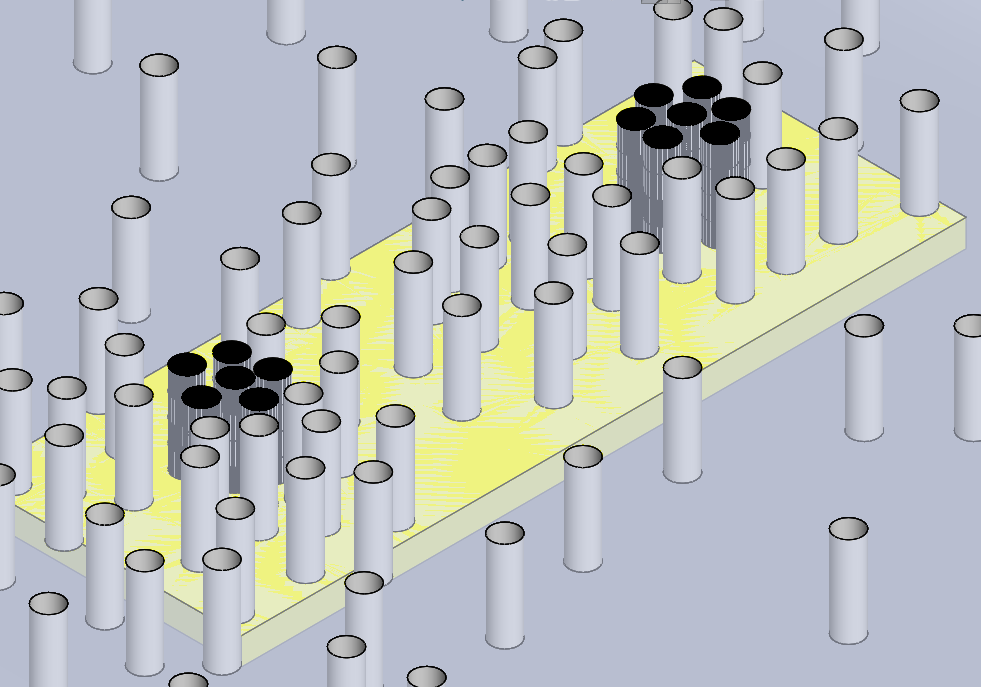
\includegraphics[scale = 0.27]{assets/figures/ED.png}
                  \caption{Électrodépositions effectuées un côté après l'autre}
              \end{subfigure}
              \begin{subfigure}{0.45\textwidth}
                  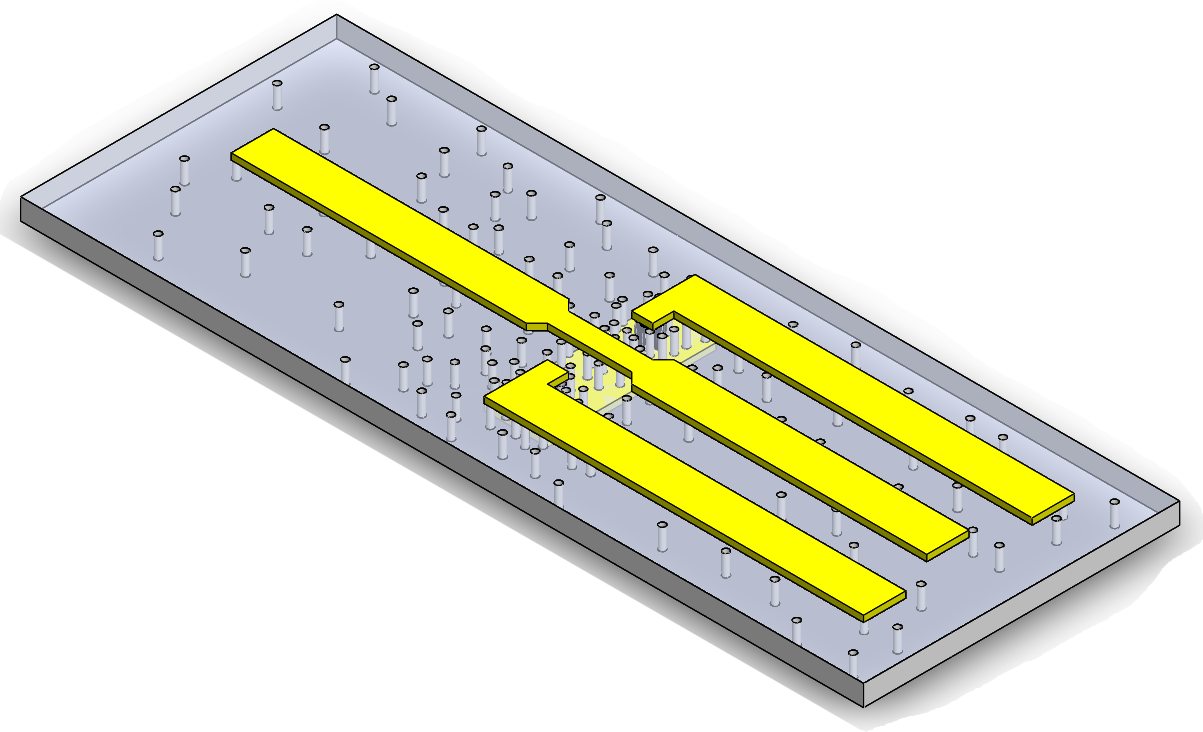
\includegraphics[scale = 0.27]{assets/figures/PVD_L.png}
                  \caption{PVD d'or des branches en L}
              \end{subfigure}
          \end{figure}
          
          \noindent \begin{enumerate}[label=(\alph*), wide, labelwidth=!, labelindent = 0pt]
              \item C'est à partir d'une membrane nanoporeuse qu'un capteur est fabriqué. Les différentes membranes sont listées dans le tableau
                    \ref{tab:membranes}. \\
              \item Une première \gls{pvd} est effectuée. De l'or vient être déposé grâce à un masque en forme de bande.
                    Cette couche d'or servira de court-circuit pour le capteur. \\
              \item Par la suite, vient l'étape des électrodépositions. Une première électrodéposition vient remplir les nanopores de la membrane
                    sur un côté du court-circuit. L'électrodéposition se fait au sein de toutes les nanopores dans un diamètre défini (nommé diamètre du via). 
                    Les nanofils se forment depuis la couche d'or de court-circuit et s'accroissent jusqu'à atteindre l'autre face de la membrane. 
                    Puis une seconde électrodéposition se fera, de la même manière, de l'autre côté de la couche d'or du court-circuit. \\
              \item La dernière étape de cette méthode consiste à effectuer une \gls{pvd} sur l'autre face de la membrane. Cette \gls{pvd} formera
                    le circuit du thermocouple complet ainsi que le corps de chauffe (au centre). 
          \end{enumerate}
          
          \newpage
    \item \textbf{Méthode B}
          \begin{figure}[H]
              \centering
              \begin{subfigure}{0.45\textwidth}
                  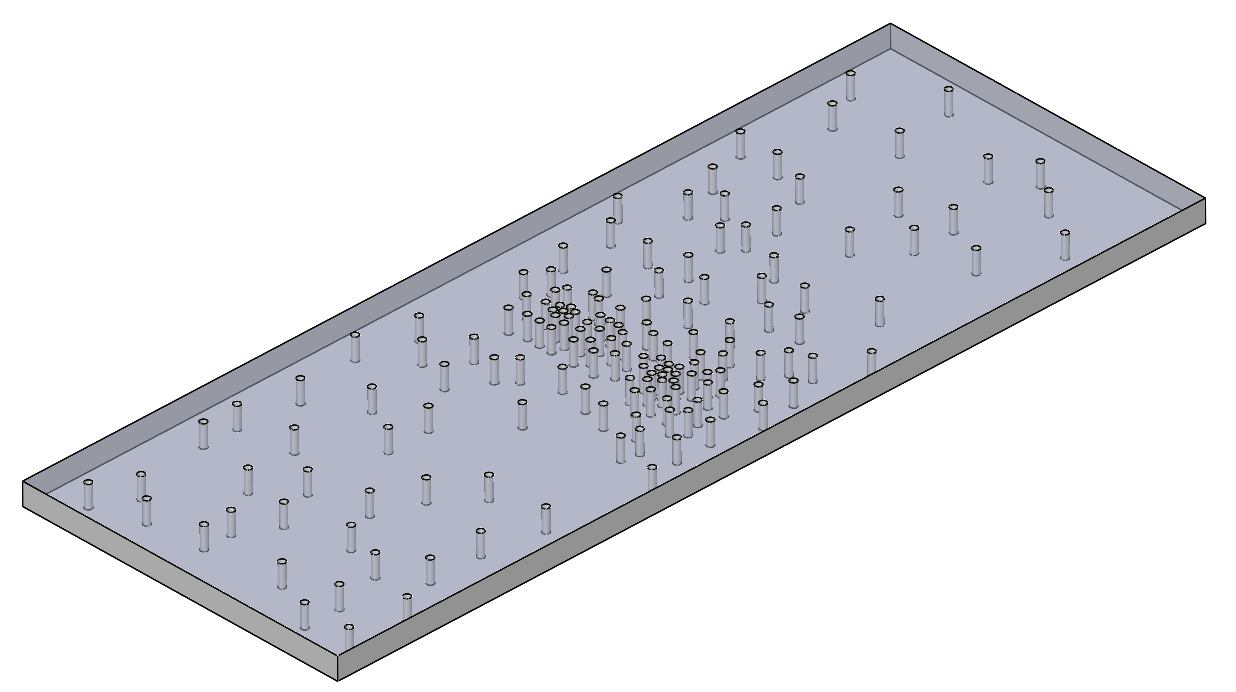
\includegraphics[scale = 0.27]{assets/figures/Membrane_nue_B.png}
                  \caption{Membrane nanoporeuse}
              \end{subfigure}
              \begin{subfigure}{0.45\textwidth}
                  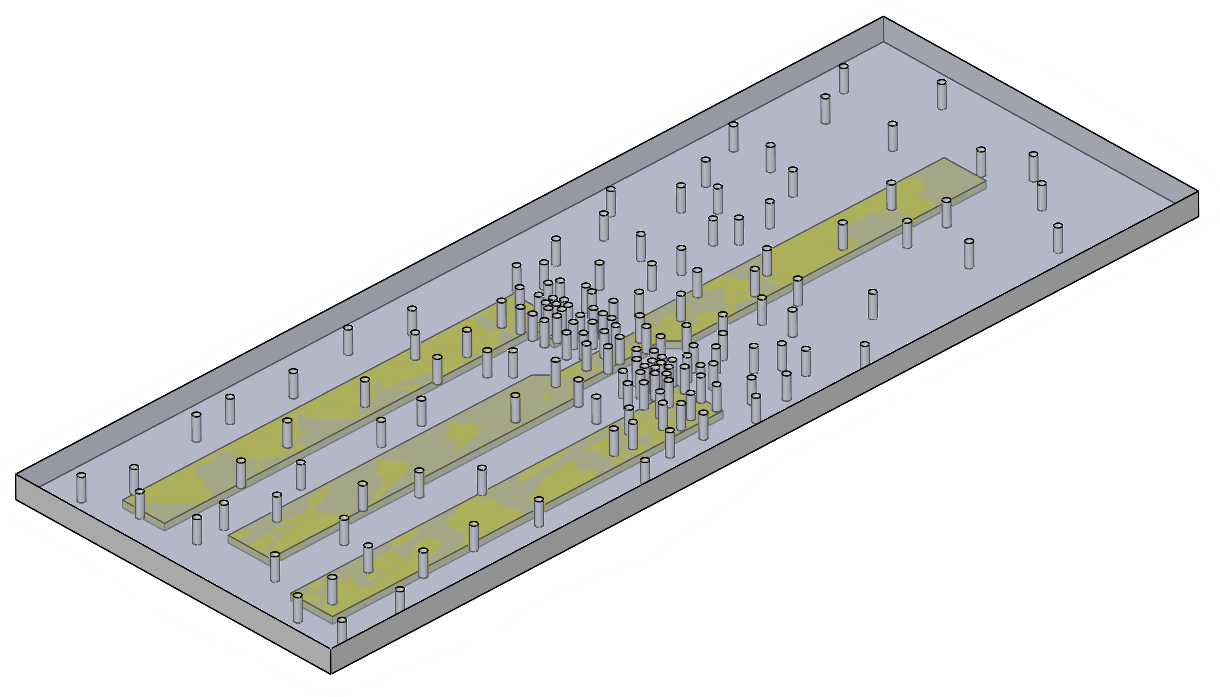
\includegraphics[scale = 0.27]{assets/figures/PVD_L_B.png}
                  \caption{PVD d'or des branches en L}
              \end{subfigure}
              \newline
              \begin{subfigure}{0.45\textwidth}
                  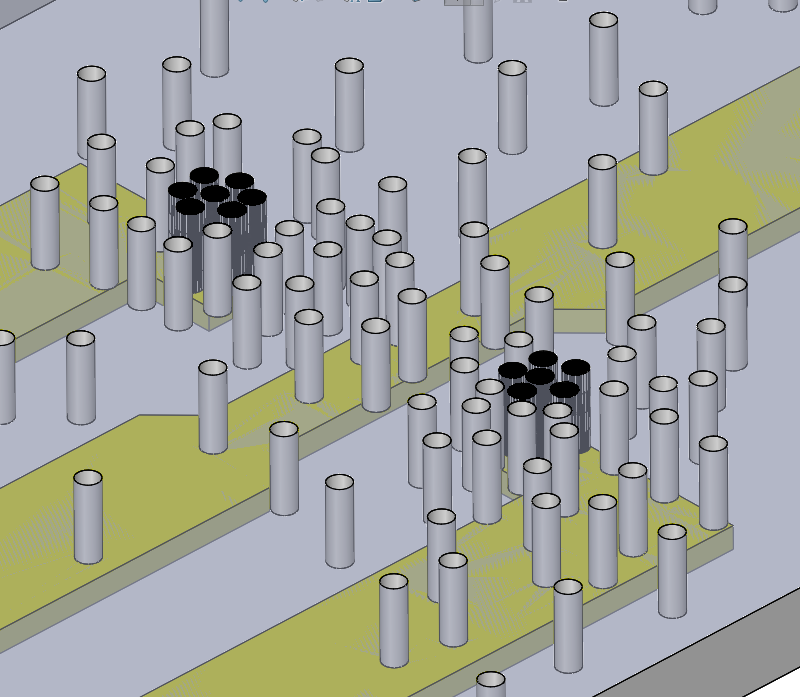
\includegraphics[scale = 0.27]{assets/figures/ED_B.png}
                  \caption{Électrodépositions effectuées une après l'autre}
              \end{subfigure}
              \begin{subfigure}{0.45\textwidth}
                  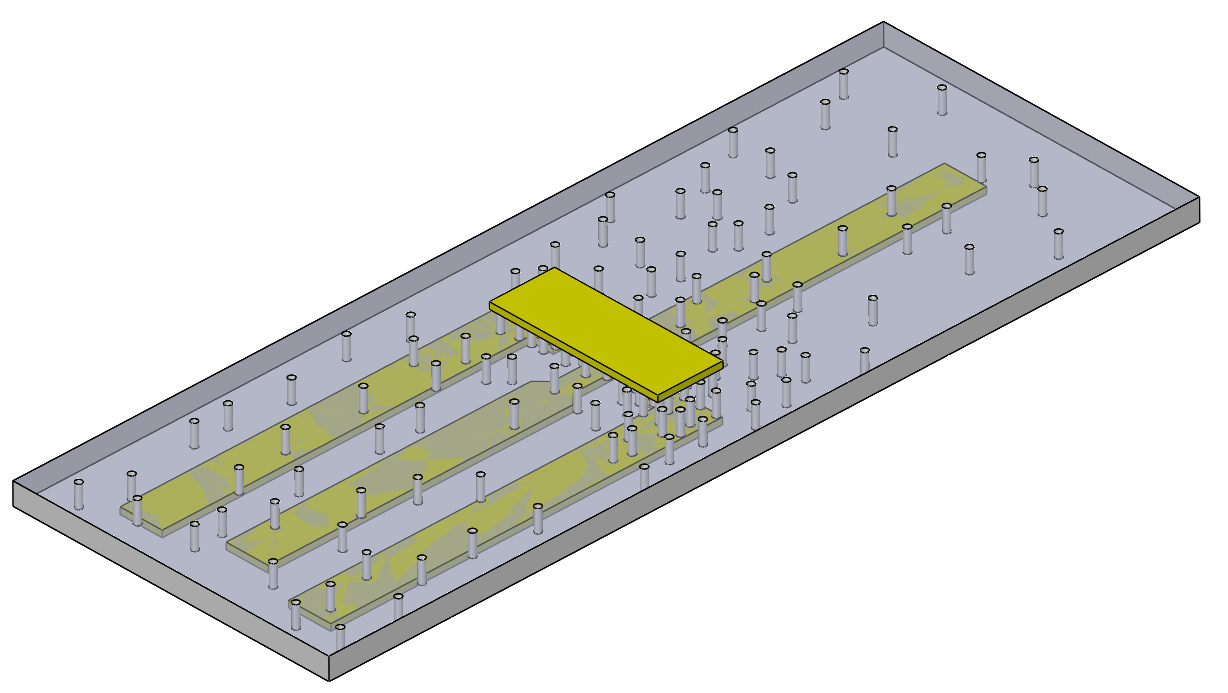
\includegraphics[scale = 0.27]{assets/figures/Court_circuit_B.png}
                  \caption{PVD d'or du court-circuit}
              \end{subfigure}
          \end{figure}
          \begin{enumerate}[label=(\alph*), wide, labelwidth=!, labelindent = 0pt]
              \item La première étape de cette méthode est également l'acquisition de la membrane nanoporeuse souhaitée.\\
              \item La première \gls{pvd} de cette méthode est la déposition des couches d'or en forme de "L" et du corps de chauffe.\\
              \item Puis, vient l'étape des électrodépositions. Une première électrodéposition vient remplir les nanopores de la membrane sur une
                    des extrémités en forme de "L". Les nanofis se forment depuis la couche d'or en forme de "L" et s'accroissent jusqu'à 
                    atteindre l'autre face de la membrane. Puis une seconde électrodéposition se fera, de la même manière, sur l'autre piste d'or 
                    en forme de "L".\\
              \item La deuxième \gls{pvd} se fait sur l'autre face de la membrane. Cette \gls{pvd} formera la piste de court-circuit du thermocouple.
          \end{enumerate}
\end{itemize}

\newpage
\subsection{Surcroissances en méthode A et B}
Les méthodes présentées au chapitre précédent engendrent chacune une certaine configuration du capteur. 
\begin{figure}[H]
    \hspace{-0.1cm}
    \begin{subfigure}{0.45\textwidth}
        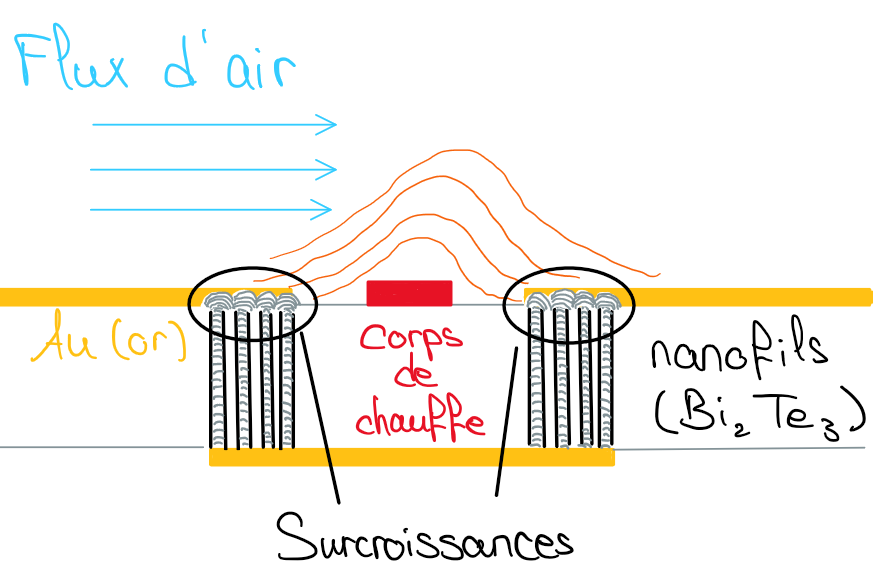
\includegraphics[scale = 0.4]{assets/figures/Methode_A_surcroissances.png}
        \caption{Surcroissances en méthode A}
    \end{subfigure}
    \hspace{0.7cm}
    \begin{subfigure}{0.45\textwidth}
        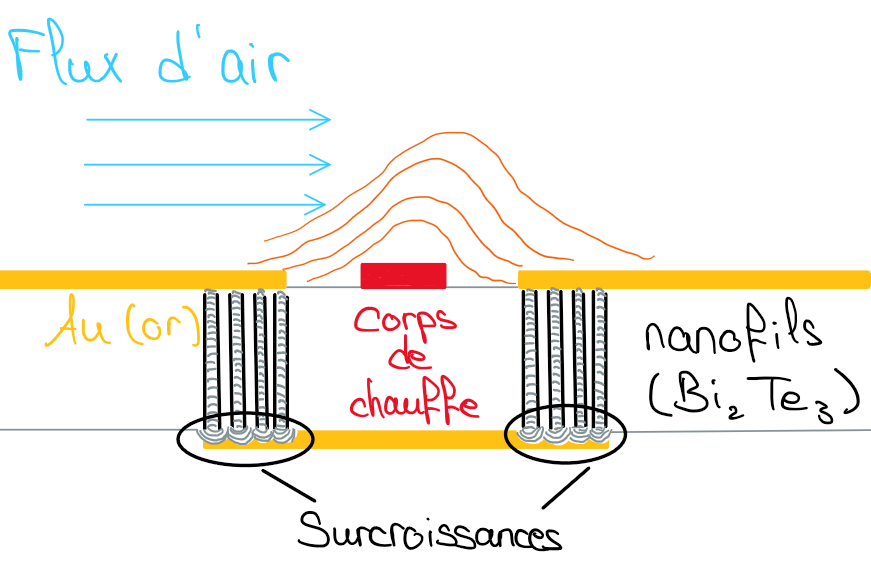
\includegraphics[scale = 0.4]{assets/figures/Methode_B_surcroissances.png}
        \caption{Surcroissances en méthode B}
    \end{subfigure}
    \caption{Surcroissances méthode A vs méthode B}
\end{figure}
Les surcroissances entraînées par l'\gls{ed} ne se retrouveront pas au même endroit suivant la méthode utilisée. En effet, lors de la méthode A 
les surcroissances sont situées au niveau des pistes d'or en "L" tandis que pour la méthode B, ces surcroissances se situent au niveau de la piste 
d'or du court-circuit. 

\subsection{Dénomination des échantillons}
\begin{table}[H]
    \centering
    \begin{tabular}{|c|c|c|}
        \hline
        Échantillon & Membrane & Méthode d'électrodéposition \\
        \hline
        D06         & GTTP     & A                           \\
        \hline
        D12         & PI25005  & A                           \\
        \hline
        D13         & PI25005  & B                           \\
        \hline
        D14         & VCTP     & A                           \\
        \hline
    \end{tabular}
    \caption{Dénomination des échantillons}
\end{table}

\newpage
\section{Catalogue des solutions du support}
\label{chap:catalogueSol}
Plusieurs systèmes ont été étudiés afin d'incorporer le capteur dans une conception permettant de connecter les membranes et le corps de chauffe
ainsi que d'y attacher un système apportant un flux d'air (imitation de la respiration du patient). Ces différentes solutions seront appelées
"Support des capteurs \gls{capteur}s".

\subsection{Solution 1}
\begin{figure}[H]
    \centering
    \begin{subfigure}{0.45\textwidth}
        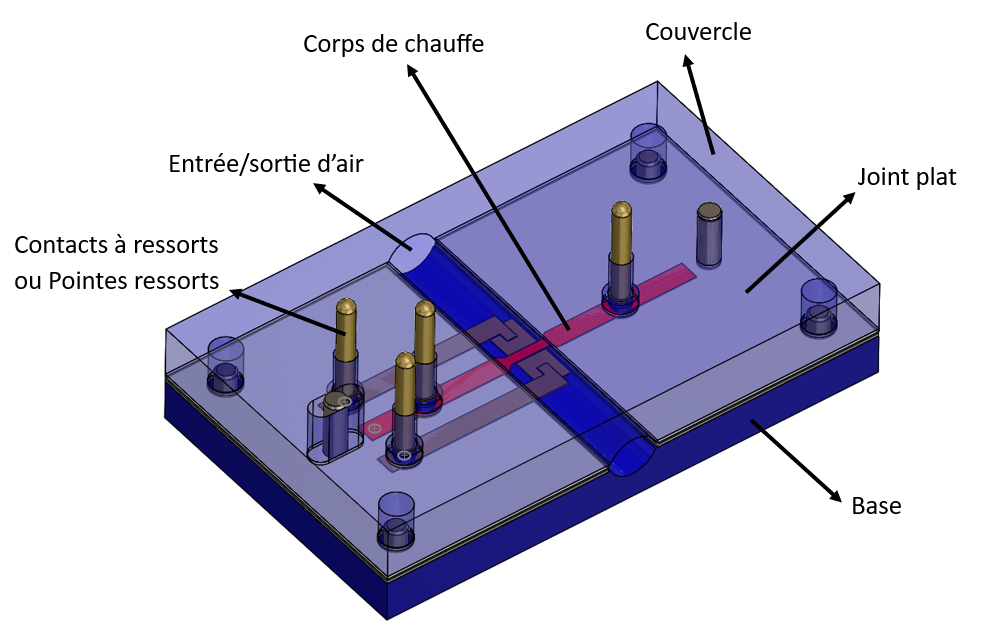
\includegraphics[scale = 0.4]{images/Design1_dessus.png}
        \caption{Vue de dessus}
    \end{subfigure}
    \hspace{1.3cm}
    \begin{subfigure}{0.45\textwidth}
        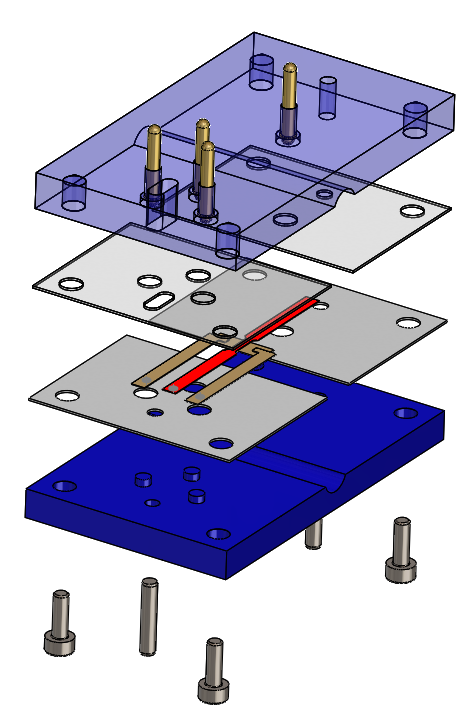
\includegraphics[scale = 0.45]{assets/figures/design1_eclate.png}
        \caption{Vue éclatée de dessus}
    \end{subfigure}
    \caption{Support 1}
    \label{fig:solution1}
\end{figure}

\begin{figure}[H]
    \centering
    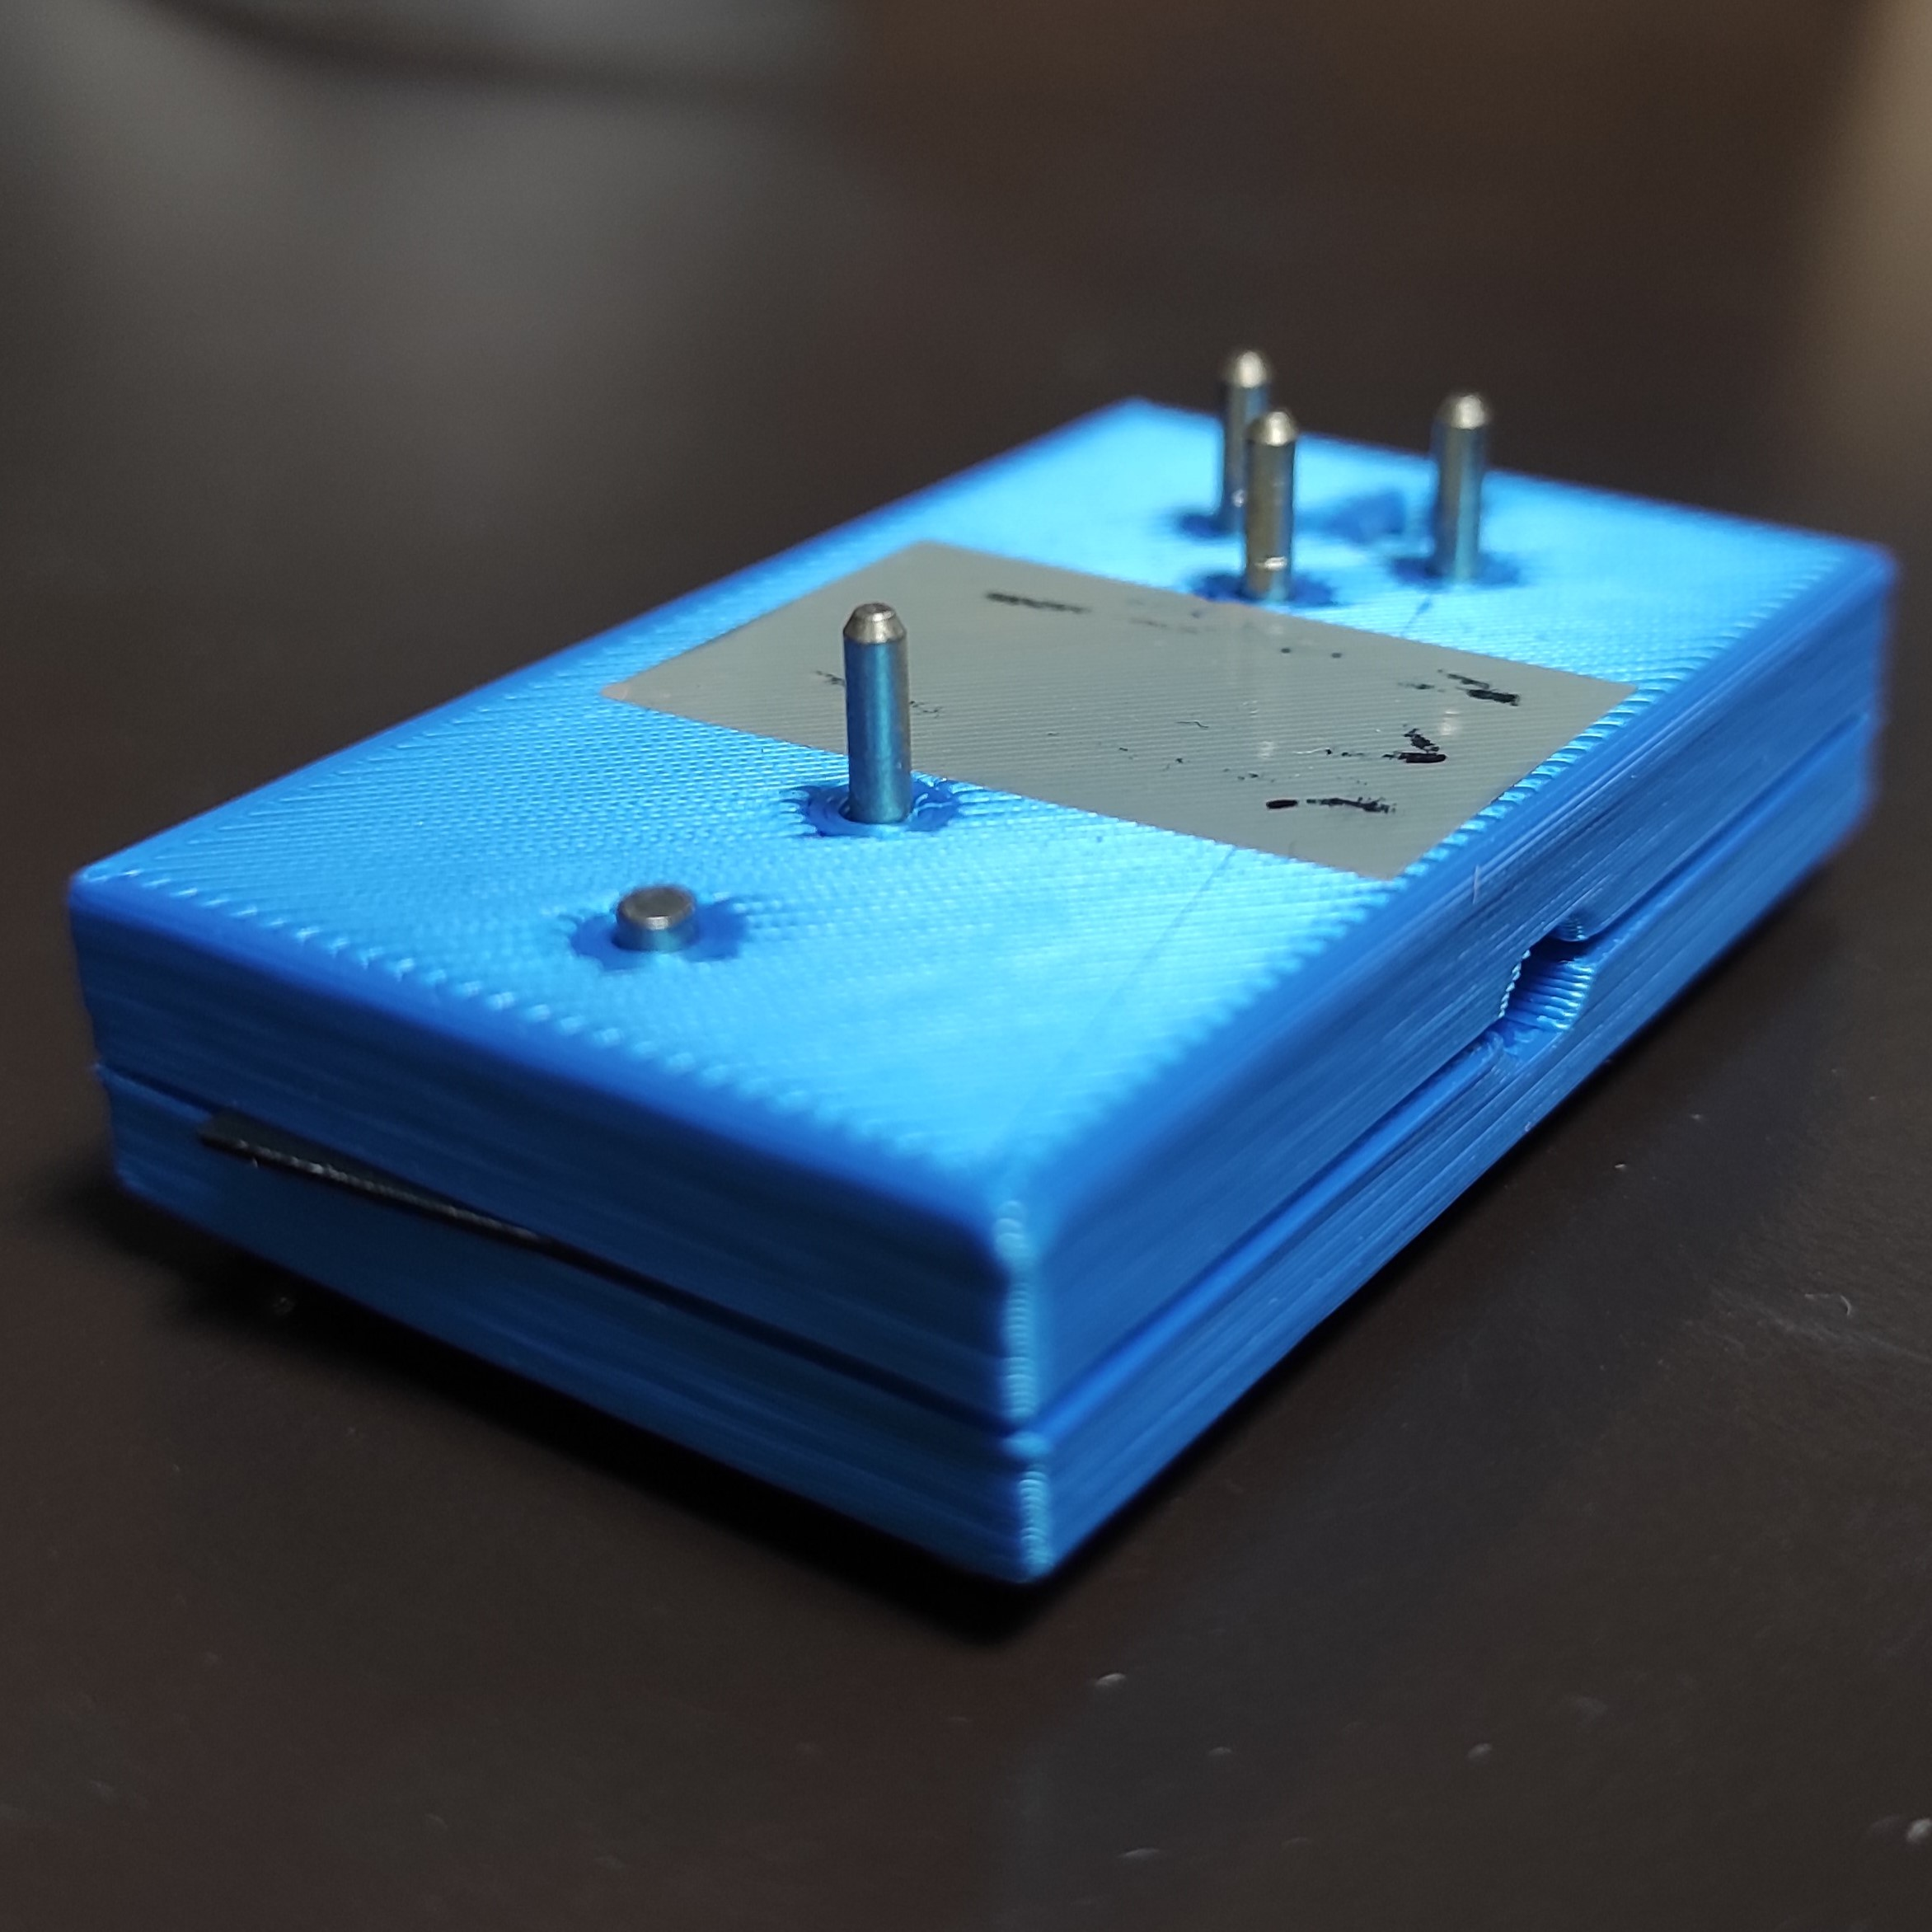
\includegraphics[scale = 0.05, angle = 0]{assets/figures/Blue_real.jpg}
    \caption{Image réelle du support 1}
\end{figure}

Cette première solution est la plus basique. Elle vient plaquer le capteur entre deux pièces presque semblables. Sur le couvercle se trouve des
perçages permettant de tenir des contacts à ressorts (pointes ressorts). Ceux-ci viennent s'appuyer d'un côté sur le capteur et
de l'autre, une  connexion pourra être faite par des pinces crocodiles ou des soudures. \\
Un joint plat peut venir de part et d'autre du capteur afin d'assurer l'étanchéité du système.\\
Cette solution a le désavantage d'avoir une arrivée d'air scindée en deux. Le placement ainsi que l'étanchéité au niveau de l'entrée
d'air risque d'être mauvaise. \\
Ceci mis de côté, c'est une solution simple, rapide et compacte.

\newpage
\subsection{Solution 2}
Afin d'éviter l'entrée d'air scindée en deux, une solution pourrait être celle représentée ci-dessous :
\begin{figure}[H]
    \centering
    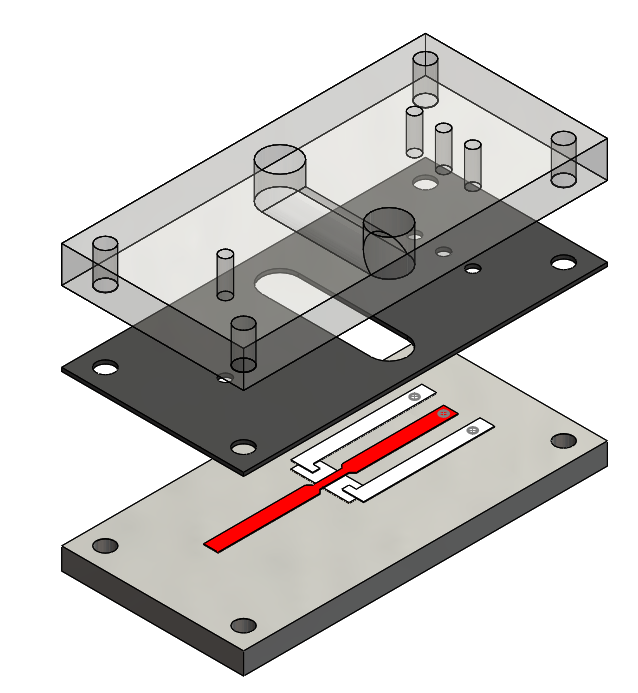
\includegraphics[scale = 0.4]{assets/figures/design2_eclate.png}
    \caption{Support 2}
    \label{fig:solution2}
\end{figure}
L'arrivée d'air se fait par le haut du système et est dévié par la suite afin d'arriver sur le capteur. Cette solution permet d'avoir une
entrée d'air plus solide que la solution précédente avec l'utilisation, par exemple d'un raccord pneumatique. Cependant, elle ajoute un risque 
non négligeable au niveau des turbulences. En effet, les coudées risquent d'engendrer des turbulences au niveau du flux qui pourraient altérer 
les résultats.\\
Une particularité à noter est le fait que la membrane se retrouve entièrement plaquée contre la base contrairement à la solution
précédente où le centre de la membrane (là où sont situés les \gls{ed}), est suspendu.

\subsection{Solution 3}
Une manière de diminuer les turbulences seraient d'élargir le système afin que les coudées ne se retrouvent pas trop proches de la
membrane. Cette solution est illustrée par la figure \ref{fig:solution3}. 

\begin{figure}[H]
    \centering
    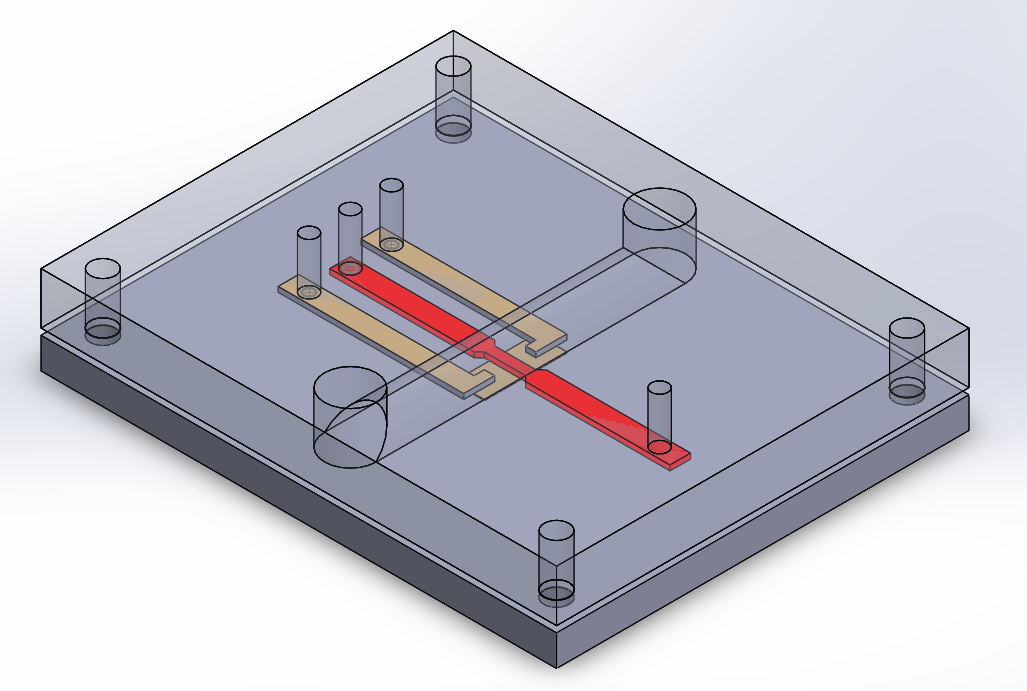
\includegraphics[scale = 0.3]{images/Design4}
    \caption{Support 3}
    \label{fig:solution3}
\end{figure}
Cette solution a le désavantage d'augmenter l'encombrement général du capteur et ne garanti pas de supprimer totalement les turbulences. 


\begin{comment}
\section{Solution 4}
Une autre manière d'éviter ce problème de turbulences et de changer la conception. Ainsi, le capteur pourrait être fabriqué selon la
figure \ref{fig:solution6}.

\section{Solution 4}%à effacer
\begin{figure}[H]
    \centering
    \includegraphics[scale = 0.5]{images/Solution6}
    \caption{}
    \label{fig:solution6}
\end{figure}

Cependant, cette solution engendre un nombre de pièces plus élevé que les solutions précédentes. En effet, pour une conception comme celle
de la figure \ref{fig:solution6}, 4 pièces seraient nécessaires contre 2 pièces pour les solutions précédentes.\\
Deux pièces viendraient pincer le capteur en sandwich comme montré pour la solution 1, figure \ref{fig:solution1}, puis, deux autres pièces
viendraient se poser sur les deux longueurs du système afin de permettre de connecter facilement une arrivée d'air.
\end{comment}

\newpage
\subsection{Solution 4}
Finalement, une dernière conception a été imaginée :
\begin{figure}[H]
    \centering
    \begin{subfigure}{0.45\textwidth}
        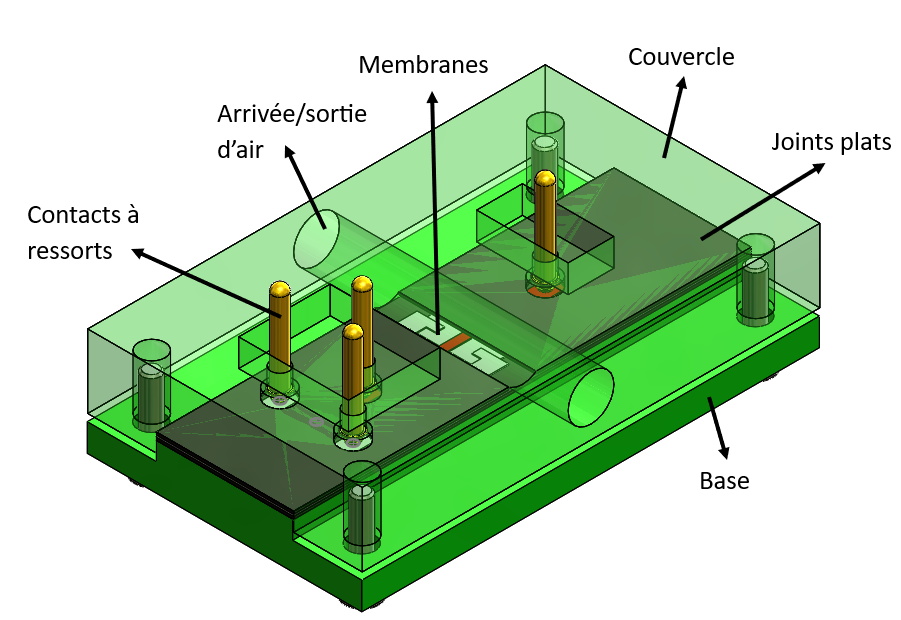
\includegraphics[scale = 0.4]{images/Design5_dessus.png}
        \caption{Vue de dessus}
    \end{subfigure}
    \hspace{1.5cm}
    \begin{subfigure}{0.3\textwidth}
        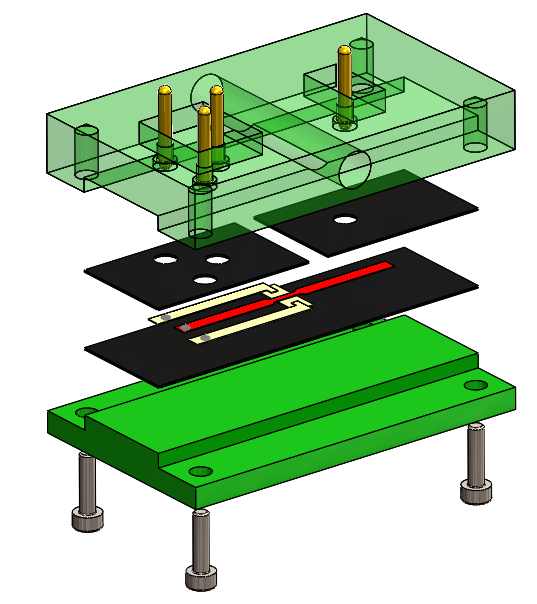
\includegraphics[scale = 0.45]{assets/figures/designSol4_eclate.png}
        \caption{Vue éclatée de dessus}
    \end{subfigure}
    \caption{Support 4}
    \label{fig:solution4}
\end{figure}

\begin{figure}[H]
    \centering
    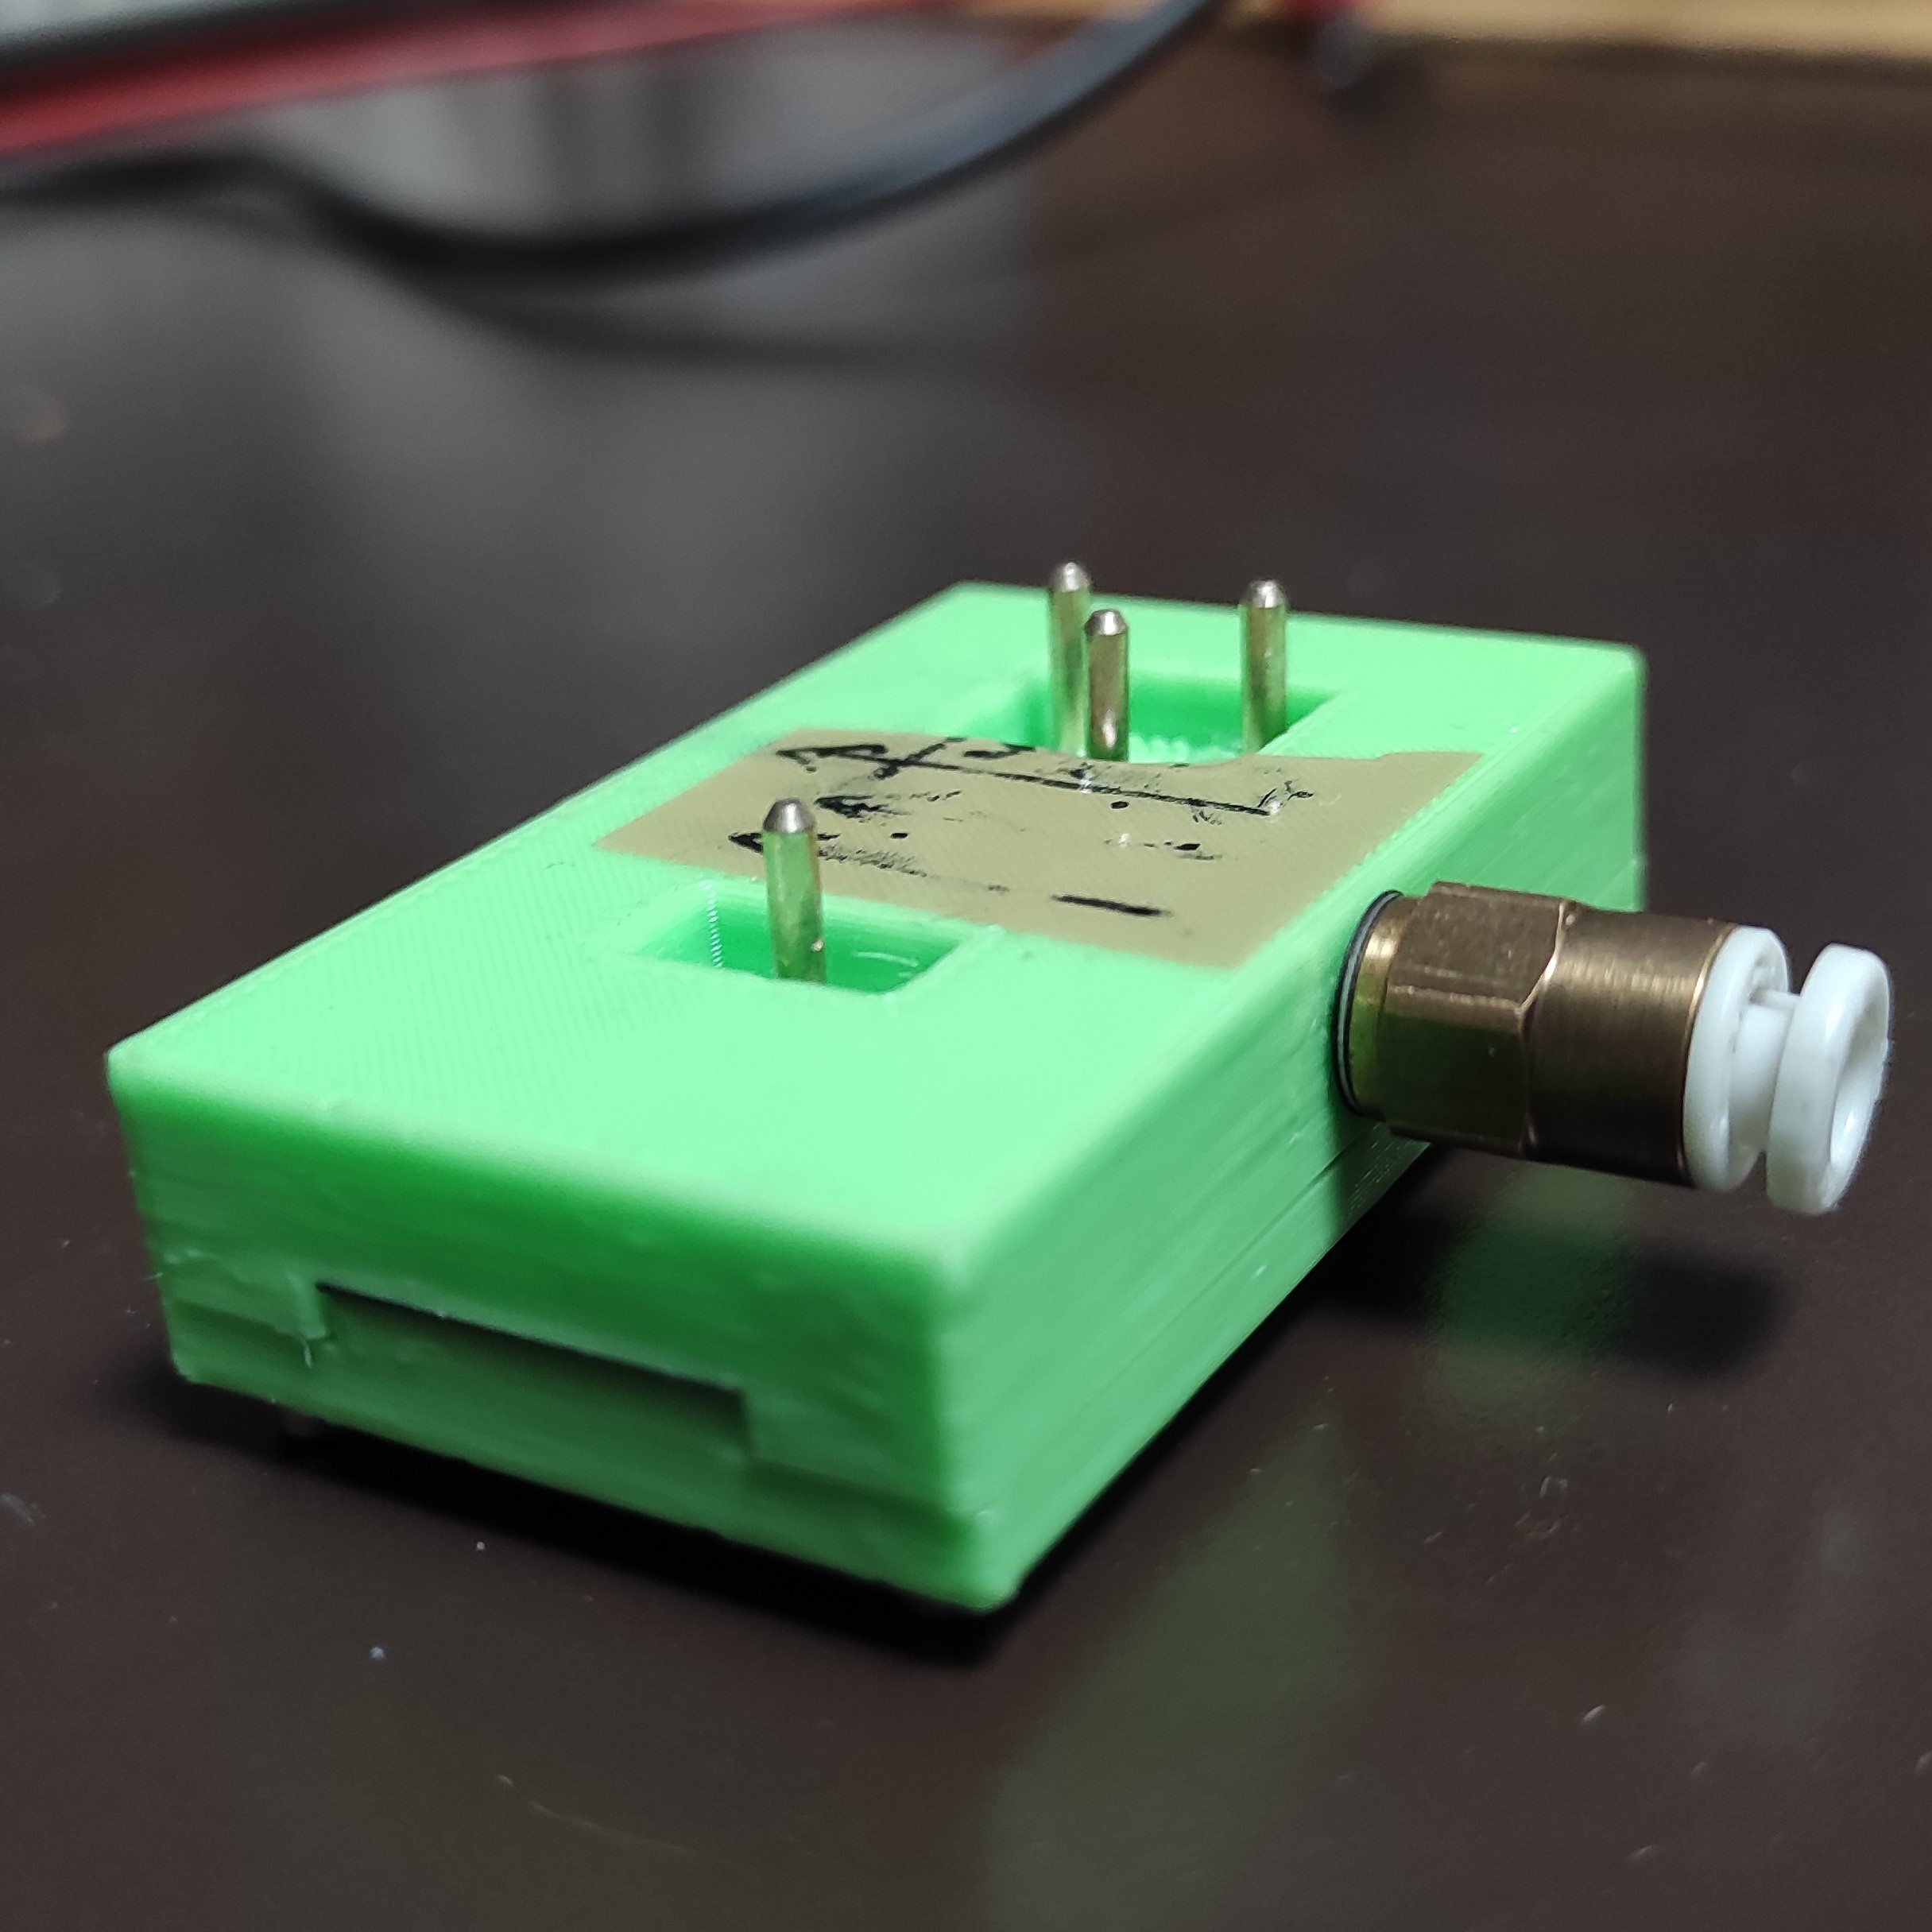
\includegraphics[scale = 0.05]{assets/figures/Green_real.jpg}
    \caption{Image réelle du support 4}
\end{figure}

Cette dernière garderait une entrée/sortie d'air facilitée (non scindée en deux) mais serait sans coudées (turbulences).\\
La membrane (capteur) est posée sur une surface de la base légèrement surélevée. Un joint plat d'étanchéité viendrait sur la membrane (en noir
sur la figure). Puis, un couvercle viendrait s'appuyer en sandwich contre le joint et le capteur. Ce couvercle est percé afin d'amener le flux 
d'air au niveau du capteur. Des plus petits perçages ainsi que des espaces creusés dans la pièce du dessus permettent aux pointes ressorts de 
venir se poser sur la membrane afin d'assurer la connexion électrique.\\

Finalement, deux solutions ont été retenues. Le support 1 (représenté en bleu) ainsi que le support 5(représenté en vert). Ces deux solutions vont être testées afin de mesurer la
performance d'un capteur recevant un flux d'air depuis le haut et depuis le bas simultanément ainsi qu'un capteur ne recevant un flux
d'air seulement par le haut (car le capteur est plaqué contre une surface).